%\documentclass[authoryear,round]{tufte-book}
\documentclass[a4paper,10pt]{article}
\usepackage[T1]{fontenc}
\usepackage[utf8]{inputenc}
\usepackage{amsmath,mathrsfs}
\usepackage{amssymb}
\usepackage{graphicx}
\usepackage{fullpage}
\usepackage{color}
\usepackage{natbib}
\usepackage{mathrsfs}
\usepackage{array}
\newcommand{\head}[2]{\multicolumn{1}{>{\centering\arraybackslash}p{#1}}{#2}}
%\usepackage{sidecap}
\usepackage[capbesideposition={top,right},facing=yes,capbesidesep=quad]{floatrow}
\usepackage[hypertexnames=false]{hyperref}
\hypersetup{colorlinks=true, urlcolor=blue, citecolor=black, linkcolor=black}
%\usepackage{lineno}
%\usepackage{lscape}
%\usepackage{multirow}

\newcommand{\var}{\mathop{\mbox{Var}}}
\newcommand{\cov}{\mathop{\mbox{Cov}}}
\newcommand{\fancyN}{$\mathcal N$ }
\newcommand{\fancyB}{$\mathcal B$ }
\newcommand{\gc}[1]{{\it \color{red} (#1)} }
\newcommand{\jb}[1]{{\it\color{blue} (#1)} }
\def\citeapos#1{\citeauthor{#1}'s (\citeyear{#1})}
%\newcommand{\Rho}{\mathrm{P}}

%opening

\title{A Coalescent Model of a Sweep from a Uniquely Derived Standing Variant}

\author{
Jeremy J. Berg$^{1,2,3}$ and Graham Coop$^{1,2,3}$ \\
$^1$ Graduate Group in Population Biology, University of California, Davis. \\
$^2$ Center for Population Biology, University of California, Davis.\\
$^3$ Department of Evolution and Ecology, University of California, Davis\\
\small To whom correspondence should be addressed: \texttt{jjberg@ucdavis.edu, gmcoop@ucdavis.edu}\\
}

\date{}

\begin{document}

%\linenumbers
\maketitle

\begin{abstract}
Understanding the impact of positive directional selection on patterns of genetic and phenotypic diversity 
\end{abstract}

%%%%%%%%%%%%%%%%%%%%%%%%%%%
\section*{Introduction}

In recent decades, an understanding of how positive directional selection and the associated hitchhiking effect influence patterns of genetic variation has become a valuable tool for evolutionary geneticists. The reductions in genetic diversity and long extended haplotypes that are characteristic of a recent selective sweep can allow for both the identification of individual genes that have contributed to recent adaptation within a population (i.e. hitchhiking mapping), and for understanding the rate and dynamics of adaptation at a genome-wide level \citep{Wiehe:1993th,Andolfatto:2007cq,EyreWalker:2009fq,Elyashiv:2014uc}.

While the contribution of many different modes to the adaptive process has long been recognized \jb{REFS}, early work on the hitchhiking effect focused largely on the scenario where a single co-dominant mutation arose and was immediately beneficial, rapidly sweeping to fixation \citep{Smith1974,Kaplan1989}. Both simulation studies and analytical explorations during the last decade however have drawn attention to alternate sweep model in which multiple independent copies of the beneficial allele may be present in the standing variation or arise from recurrent mutation before the sweep has completed \citep{Innan:2004bk,Przeworski2005,Hermisson2005,Pennings2006a,Pennings2006,Hermisson2008,BARRETT:2008cs,Ralph2010,Pokalyuk2012,Roesti:2014gp,Wilson:2014ke}. Collectively, these phenomena have come to be known as ``soft sweeps'', a term originally coined by \cite{Hermisson2005}, and now often used \gc{as a catchall phrase} to refer to any sweep for which the most recent common ancestor at the locus of the beneficial allele(s) predates the onset of positive selection \citep{Messer:2013kh}. 

Empirical work occurring largely in parallel with the theory discussed above suggests that soft sweeps of one variety or another likely make a substantial contribution to adaptation. For example, many freshwater stickleback populations have independently lost the bony plating of their marine ancestors due to repeated selection on an ancient standing variant at the \textit{Eda} gene \citep{Colosimo:2005ee}, and a substantial fraction of the increased apical dominance in maize relative to teosinte can be traced to a standing variant which predates domestication by at least 10,000 years \citep{Studer:2011bya}. Additional examples of adaptation from standing variation have been documented in \textit{Drosophila} \citep{Magwire:2011eq}, \textit{Peromyscus} \citep{Domingues:2012kw} and humans \citep{Peter:2012ht}, among others. Adaptations involving simultaneous selection on multiple alleles of independent origin at the same locus have also been documented across a wide array of species \citep{Menozzi:2004iu,Nair2007,Karasov:2010ij,Salgueiro:2010hx,Schmidt:2010bu,Jones:2013iw}. Nonetheless, the general importance of soft sweeps for the adaptive process remains somewhat contentious \citep[see e.g.][]{Jensen:2014hd}.

While models of the hitchhiking effect under soft sweeps involving multiple independent mutations have received a fair amount of analytical attention \citep{Pennings2006a,Pennings2006,Hermisson2008,Pokalyuk2012,Wilson:2014ke}, the model of a single origin mutation which segregates as a standing variant before sweeping in response to an environmental change is less well characterized. Present understanding of the hitchhiking effect in a single population under this model comes primarily from two sources. The first is a pair of simulation studies \citep{Innan:2004bk,Przeworski2005}, which focused largely on simple summaries of diversity and the allele frequency spectrum, and the second is the general verbal intuition that, similar to the multiple mutation case, the beneficial allele should be found on ``multiple haplotypes''. In contrast to the multiple mutation case, these additional haplotypes are created as a result of recombination events during the period before the sweep when the allele was present in the standing variation, rather than due to recurrent mutations on different ancestral haplotypes \citep{BARRETT:2008cs,Messer:2013kh}.

In this paper, we present an analytical treatment of this model in which an allele with a single mutational origin segregates at low frequency (either neutrally or under the influence of balancing selection with asymmetric heterozygote advantage) and then sweeps to fixation after a change in the environment. The central observation is that, with some simplifying assumptions, the recombination events which are responsible for the multiple haplotypes on which the beneficial allele is found have a close analogy to mutations in the infinite alleles model, and we can therefore leverage the Ewens Sampling Formula to obtain an analytical description for the genealogical history of a neutral locus linked to the beneficial allele. We then show that this model can be used to obtain a highly accurate approximation for the expected deviation in the frequency spectrum at a given genetic distance, as well as to shed light on how the expected pattern of haplotype structure differ between the multiple recurrent mutation and sweep from standing  variation cases. We conclude with a brief simulation study examining the order statistics of the haplotype frequency spectrum under the classic hard sweep, multiple mutation soft sweep, and standing sweep models, with the aim of demonstrating how future methods to identify and classify sweeps can best make use of this information.
 
%
%In a subsequent pair of papers also under the ``soft sweeps'' banner, they focused on a slightly different scenario, in which new mutations arising once a selective sweep had already begun managed to increase in frequency quickly enough to make a substantial contribution to a class of beneficial alleles before the first sweeping mutation has managed to fix. In the usage of Pennings and Hermisson, these sweeps are ``soft'', in that they include contributions from multiple independent mutations, even though they do not come from the standing variation.
%
%Some authors, by contrast, have used a looser definition of soft sweep \jb{will have to track down citations for this; recent X v. autosome preprint about human/chimp speciation from Mailund and friends is one example}. In contrast to the definition proffered by Pennings and Hermisson, under this usage a soft sweep is generally ``a selective sweep in which the beneficial mutation is present on more than one \gc{common} haplotype'', irrespective of the histories of the beneficial mutations on those haplotypes. Under this definition, an adaptive fixation with only a single mutational origin may be considered a ``soft sweep'' if it was present as standing variation in the population before \gc{the environmental shift, e.g. if it was neutral or balanced at low frequency. In that case the allele can be been recombining on to different haplotype in the population for some time,} before a change in the environment caused it to become beneficial, at which point \gc{multiple} haplotypes onto which the beneficial mutation has recombined collectively sweep to \gc{intermediate frequencies}.
%
%\gc{
%The role of soft sweeps is shaping genome-wide patterns of variation has been debated contenious \citep{Dmitripreprint, Dmitrireive, Jensen, Pritchard, Hernandez}, and touches on a number of important questions, e.g. the extent to which adaptation is mutation-limited. However, while the term soft sweep is catchy it is likely also (likely) unhelpfully broad and may lead to confusion \gc{(and we have likely been guilty of adding to this ourselves)}. While a variety of models lead to violations of the simple sweep pattern, they do not leave identical patterns and differ strongly in the decay of their signal as we move away from the selected site (as we discuss below). We think it best to be more specific and call these different models a ``sweep from multiple mutations'' or a ``sweep from a single standing variant''. In practice it can be hard to distinguish these various kinds of sweeps, and often hard to distinguish them from hard sweeps, but it is a useful distinction to make. }
%
%Further confusing the situation, selection on recessive alleles can also lead to 
%
%
%\jb{this transition is really clunky and needs to be fleshed out more}
%
%\gc{The model of a ``sweep from a single standing variant'' has} been studied via simulation by previous authors such as \cite{Innan:2004bk} and \cite{Przeworski2005}, but to our knowledge there have been no detailed analytical investigations of the hitchhiking process of a single identical by descent mutation that sweeps after first drifting to appreciable frequency. It is this model that is the primary focus of this paper. We first develop a coalescent based approximation to describe the genealogical history of a sample taken at a locus where a beneficial allele that was previously drifting neutrally has just fixed in the population. We then consider a second neutral locus linked to this selected locus and show that a form of the Ewens Sampling Formula can be used in order to understand the hitchhiking effect at this locus, and thus to describe the expected patterns of genetic diversity surrounding a selective sweep from standing variation. Although an explicit, formal description of the haplotype frequency spectrum surrounding a sweep from standing variation is beyond our mathematical means, we show that our model can be used to gain considerable intuition into which features of it are informative, and to guide future efforts to develop inference techniques that can identify sweeps from standing variation as well as distinguish among different varieties. Lastly, although our model is primarily motivated by the case of a neutral or balanced polymorphism that eventually becomes beneficial and sweeps, we show that our model also provides an adequate description of the hitchhiking signature of a completely recessive sweep (either \textit{de novo} or from standing variation \jb{obv need to explore this more, but have a hunch that recessive mutation that was previously at mut-sel balance will be fit well by our model}), for reasons that are relatively easy to explain \jb{note: explain them}.
%
\section*{Model}

%\subsection{more technical}

We consider two linked loci separated on the chromosome by a recombination distance $r$. At one of these loci a new allele, \textbf{B}, arises in a background of ancestral \textbf{b} alleles. This allele segregates at low frequency for some period of time (either due to neutral fluctuations, or because it is a balanced polymorphism), before a change in the environment causes it to become beneficial and sweep to fixation. A schematic depiction of the model is given in Figure \ref{cartoon_fig_2}. Our aim is to describe some features of genealogies both at the locus of the \textbf{B} allele and nearby linked sites, and to use this understanding to build intuition regarding the process of a sweep from standing variation, as well as to derive the patterns of DNA sequence variation we expect to observe near a recently completed sweep from standing variation.

Our general approach is to break the history of the standing sweep into two periods, the first being the time during which the B allele is selectively favored and rising in frequency (we refer to this as the sweep phase), and the second being the period after the mutation has arisen but before the environmental shift causes it to become beneficial (we refer to this as the standing phase). We assume that the frequency trajectory of the allele is logistic during the sweep phase, and that selection is sufficiently strong relative to the sample size such that only recombination (i.e. no coalescence) occurs during this phase. We approximate the standing phase by assuming that the frequency of the B allele is held at some constant value $f$ infinitely far into the past prior to the onset of selection. While this is obviously a coarse approximation to the true history of a low frequency allele, it is nonetheless accurate enough for our purposes, and enjoys some theoretical justification, as we discuss below. The key advantage to using this approximation is that it allows us to model the genealogy of the B alleles as a standard neutral coalescent (rescaled by a factor $f$), and therefore to treat recombination events moving away from the selected locus in a manor analogous to mutations in the standard infinite alleles model. This allows us to use a version of the Ewens Sampling Formula to calculate a number of summaries of sequence diversity, and to build intuition for how patterns of haplotype diversity should change in regions surrounding a standing sweep.

%\jb{In this paper, we will use the phrase `beneficial allele' to refer to the allele that becomes beneficial during the selected phase and the phrase `non-beneficial allele' to refer to the complementary allele which becomes disfavored, regardless of whether the effect of selection is actually being felt during the part of the process being considered. We will use the phrase `sweep phase' to refer to the part of the history during which the beneficial allele is increasing in frequency due to positive selection, and the phrase `standing phase' to refer to the part of the history that preceeds the onset of selection.}

\begin{figure}
	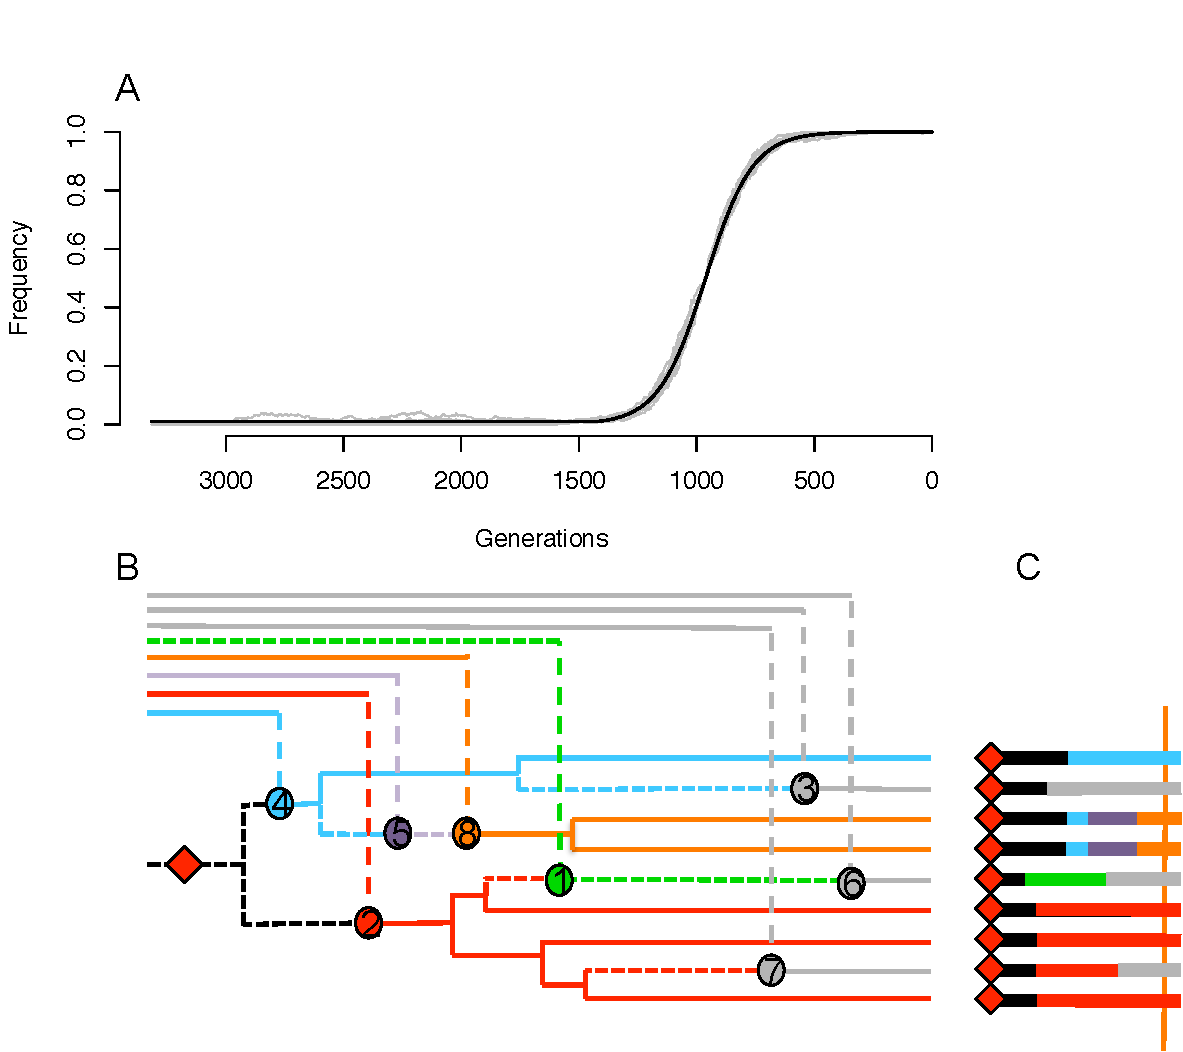
\includegraphics[width = 0.8\textwidth]{../Paper_Figures/SchematicFig1_6.pdf}
	\caption{A schematic depiction of our model. (A) Grey lines represent 10 simulated sweeps with $s=0.01$ and $f=0.01$ in a population of $N=10000$. The solid black line represents the frequency trajectory assumed for our analytical calculations. (B and C) The genealogy, history of recombination events, and sequence associated with a sample of nine chromomsomes taken at the moment of fixation. The red dot (on both the genealogy and the sequence) represents the mutation responsible for the beneficial allele. The tree subtending this mutation in panel B is the genealogy at the locus of this mutation. Solid lines represent the genealogy experienced by a neutral site located at the position of the vertical orange bar in panel C, with lineages that escape coalescence under the red mutation coalescing on a longer timescale off the left side of the figure. Stars on the genealogy in panel B represent the recombination events falling between the beneficial mutation and the orange bar in panel C, and are responsible for changes in along the sequence. Short dashed lines represent components of genealogies in between the red mutation and the orange bar which are not experienced at the position of the orange bar, while long dashed lines represent movement from the selected to the non-selected background via recombination. At the distance marked by the orange bar, there are three sweep phase recombinants, and the remaining six sequences are partitioned into three haplotypes of frequencies three, two and one, according to the infinite alleles process described in the main text.}
	\label{cartoon_fig_2}
\end{figure}

\section*{Analysis and Results}

\subsubsection*{Sweep Phase}

Looking backward in time, let $X\left(t\right)$ be the frequency of the B allele at time $t$ in the past, where $t=0$ is the moment of fixation (i.e. $X\left(0\right) = 1; X\left(t\right) < 1\ \forall\ t > 0$). If we consider a neutral locus a genetic distance $r$ away from the beneficial allele, the probability that it fails to recombine off of the selected background in generation $t$, given that it has not done so already is $1-r\left(1-X(t)\right)$. If we let $\tau_{f}$ be the generation in which the environmental change occurred, marking the boundary between the sweep phase and the standing phase (i.e. $X\left(\tau_{f}\right) = f$), then the probability that a single lineage fails to recombine off the selected background at any point during the course of the sweep phase is given by
\begin{equation}
P_{NR} = \prod_{t=0}^{\tau_{f}} 1-r\left(1-X(t)\right)  \approx \exp \left(-r \int_0^{\tau_{f}}(1-X\left(t\right))\mathrm{d} t \right) \label{P_NR}
\end{equation}
for $r \ll 1$. If the effect of our beneficial allele on relative fitness is strictly additive, such that heterozygotes enjoy a selective advantage of $s$ and homozygotes an advantage of $2s$, then the trajectory of the beneficial allele through the population can be approximated deterministically by the logistic function, and the integral in the exponential in equation \eqref{P_NR} can be approximated as $ln\left(\frac{1}{f}\right) \frac{1}{s}$, yielding
\begin{equation}
	P_{NR} \approx \exp \left(-\frac{r}{s}ln\left(\frac{1}{f}\right)\right).
\end{equation}

We assume selection is strong, such that there is not enough time for coalescence during the sweep phase. Therefore, each lineage either recombines off the beneficial background, or fails to do so, independently of all other lineages. The probability that $i$ out of $n$ lineages fail to escape off the sweeping background is then
\begin{equation}
P_{NR}(i \mid n) = {n \choose i} P_{NR}^{i} (1-P_{NR})^{n-i}.
\end{equation}
This binomial approximation has been made by a number of authors in the context of hard sweeps \citep[e.g. ][]{Smith1974,Fay:2000us,McVean:2006ke}, but better approximations do exist \citep{Barton1998,Durrett:2004fl,Durrett:2005fr,Schweinsberg:2005eh,Etheridge:2006fk,Messer:2012ie}. Under the hard sweep model, most of the error of the binomial approximation arises due to coalescent events during the earliest phase of the sweep. Because this phase is replaced in our model by the standing phase described below, the binomial approximation is a better fit for our use than in the classic hard sweep case. 


\subsubsection*{Standing Phase}
Looking backward in time, having originally sampled $n$ lineages at $t=0$, we arrive at the beginning of the standing phase at time $\tau_{f}$ with $i$ lineages still linked to the beneficial background, the other $n-i$ having recombined into the non-beneficial background during the sweep.

We apply a separation of timescales argument, noting that coalescence of the $i$ lineages which fail to recombine off the \textbf{B} background during the sweep will occur much faster than coalescence of the $n-i$ lineages which do recombine during the sweep. We therefore assume that nothing happens to lineages on the \textbf{b} background until all lineages have escaped the \textbf{B} background via either mutation or recombination, at which point \textbf{b} lineages follow the standard neutral coalescent.

%
%We will argue that an understanding of patterns of diversity at the neutral locus following a standing sweep can be obtained principally by tracking the histories of only the lineages that are found on the \textbf{B} background at the beginning of the standing phase, and assuming that lineages which recombine off of the \textbf{B} background do not re-enter it. This is obviously a coarse approximation to the true process, but as we argue below, it captures many of the major features sufficiently well for our purposes.

% The following paragraphs are therefore structured as follows: first, we describe an approximation to the coalescent process for \textbf{B} alleles at the \fancyB locus conditional on being at a frequency $f$ at the beginning of the standing phase. Next, we describe an approximation to the process of recombination events which move alleles at the \fancyN locus from the beneficial background onto the non-beneficial background at the \fancyB locus. Finally, we combine these two processes along with the recombination process during the sweep phase and a separation of timescales argument to give an approximate description of the full genealogy at the \fancyN locus.

\paragraph{The Coalescent Process of the B Alleles}

%In attempting to construct the genealogy of the B alleles backward in time, consider that in the first generation of the standing phase, the probability that any pair of B coalesces with one another is $1/\left(2Nf\right)$, while the probability that any pair of b alleles coalesce with one another is $1/\left(2N\left(1-f\right)\right)$. In general, the pairwise coalescent probabilities for pairs of lineages $T$ generations back into the standing phase are $1/\left(2NX(\tau_{f} + T)\right)$ for the B alleles, and $1/\left(2N\left(1-X\left(\tau_{f}+T\right)\right)\right)$ for the b alleles, where the frequency $X\left(\tau_{f} + T\right)$ may be equal to, greater than, or less than $f$, due to the random sampling effects of genetic drift. Further, coalescent events which may have occurred during the intervening $T$ generations contain information about the distribution of $X\left(\tau_{f} + T\right)$.

A number of previous studies have examined the behavior of this process \citep{Wiuf1999,Wiuf:2000js,Patterson2005}, either conditional on the frequency of the allele in a sample or in the population. \cite{Wiuf:2000js} has shown that the expected time to the first coalescent event is $2 N f/ {i \choose 2}$ in the absence of other information, e.g. as to whether the allele is ancestral or derived. However, the distribution of coalescence times is no longer exponential. The variance of the time between coalescent events is increased relative to the exponential as a direct result of the fact that the frequency may increase or decrease from $f$ before a given coalescent event is reached. Further, in contrast to the standard coalescent, there is non-zero covariance between subsequent coalescent intervals, as a result of the information they contain about how the frequency of the allele has changed, and thus about the rate at which subsequent coalescent events occur. Lastly, if the allele is known to be either derived or ancestral, the expected coalescent times have a more complicated expression, as the allele is in expectation either decreasing or increasing in frequency backward in time due to the conditioning on derived or ancestral status respectively.

Despite these complications, we have found that assuming that all pairs of lineages coalesce at a constant rate $1/(2 N f)$ and that coalescent time intervals are independent (in other words, that the allele frequency does not drift from $f$) is not a bad approximation when $f \ll 1$, even when we condition on the allele being derived (Figures \ref{n_2_supp_plot}, \ref{mean_coal_times_supp_plot} and \ref{coeff_var_coal_times_supp_plot}).

The main reason for using this approximation is that, in conjunction with the separation of timescales, it allows us to work with a simple, well understood caricature of the true process (i.e. the neutral coalescent) that still describes the genealogy at the selected site with reasonable accuracy. Given this simplified coalescent process, we can study the recombination events occurring between the beneficial and neutral loci to understand the properties of the genetic variation at the neutral locus that will hitchhike along with the \textbf{B} allele once the sweep phase begins.

\paragraph{Recombination Events Ocurring During the Standing Phase}

We will again rely on the condition that $f \ll 1$, and assume that any lineage at the neutral locus that recombines off of the background of our beneficial allele will not recombine back into that background before it is removed by mutation. Under these assumptions, recombination events which move lineages at the neutral locus from the \textbf{B} background onto the \textbf{b} background can be viewed simply as events on the genealogy at the beneficial locus which occur at rate $r\left(1-f\right)$ for each lineage independently. Rescaling time by $2Nf$, an understanding of the genealogy at the neutral locus can therefore be found by considering the competing poisson processes of coalescence at rate $1$ per pair of lineages, and recombination at rate $2Nrf(1-f)$ per lineage.

We are interested in the number and size of different recombinant clades at a given genetic distance from the selected site (colored clades in Figure \ref{cartoon_fig_2}B, which give rise to colored haplotypes in Figure \ref{cartoon_fig_2}C). Under our approximate model for the history of coalescence and recombination at these sites, this a direct analogy of the infinite alleles model \citep{Kimura:1964wb,Watterson:1984wb}. In the normal infinite alleles process, we imagine simulating from the coalescent, scattering mutations down on the genealogy, and then assigning each lineage to be of a type corresponding to the mutation that sits lowest above it in the genealogy. Alternately, we can create a sample from the infinite alleles model by simulating the mutational and coalescent processes simultaneously: coalescing lineages together as we move backward in time, ``killing'' lineages whenever they first encounter a mutation and assigning all tips sitting below the mutation to be of the same allelic type \citep{Griffiths:1980wy}.

Given the direct analogy to the infinite alleles model under our set of approximations, the number and frequency of the various recombinant lineage classes at a given distance from the selected site can be found using the Ewens Sampling Formula \citep{Ewens1972}. The population-scaled mutation rate in the infinitely-many alleles model ($\theta/2=2N\mu$), is replaced in our model by the rate of recombination out of the selected class ($R_{f}/2=2Nrf(1-f)$). If $i$ lineages sampled at the moment of fixation fail to recombine off of the beneficial background during the course of the sweep, then the probability that these $i$ lineages coalesce into a set of $k$ recombinant lineages is 
\begin{equation}
	p_{ESF}(k \mid R_f,n)  = S(i,k) \frac{R_f^k}{ \prod_{\ell=1}^{i-1} (R_f +\ell) }  \label{ESF1}
\end{equation}
where $S(i,k)$ is an unsigned Stirling number of the first kind
\begin{equation}
	S(i,k) = \sum_{i_1 + \dots + i_k = i} \frac{i!}{k!i_1\dots i_k}
\end{equation}
These recombinant lineages partition our sample up between themselves, such that each lineage has some number of descendants in our present day sample $\{i_1,i_2,\dots,i_k\}$, where $\sum_{j=1}^k i_j =i$. Conditional on $k$, the probability of a given sample configuration is
\begin{equation}
	p(\{i_1,i_2,\dots,i_k\} \mid k,i) = \frac{i!}{k! i_1\cdots i_k S(i,k)}  \label{ESF2}
\end{equation}
Note that this does not depend on $R_f$, which gives the classic result that the number of alleles is sufficient statistic for $R_f$ (i.e. the partition is not needed to estimate $R_f$). Figure \ref{Prob_hap_distribution} shows a comparison of this approximation to simulations for the number of distinct coalescent families at a given distance from the focal site.


\begin{figure}
	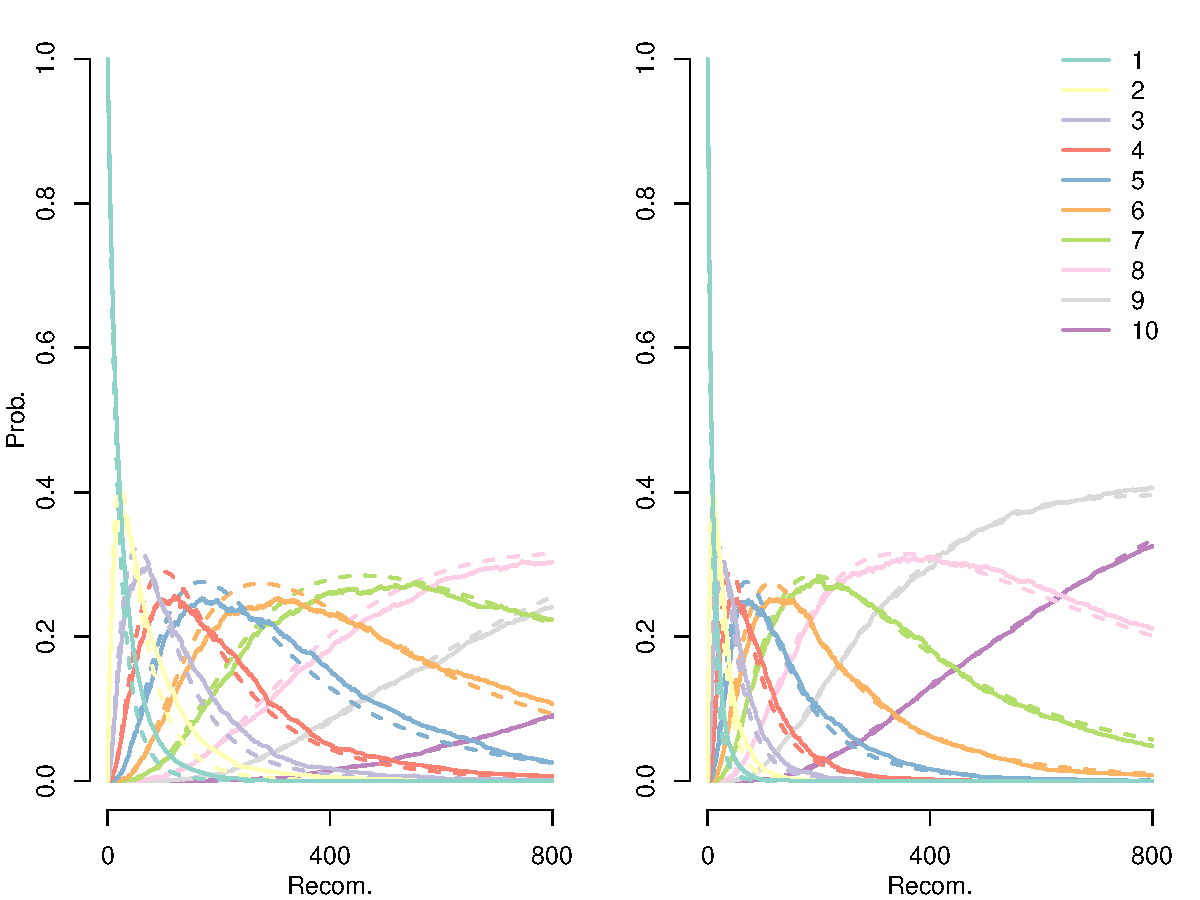
\includegraphics[width = \textwidth]{../Paper_Figures/Prob_hap_distribution.pdf}
\caption{The probability that a sample of 10 lineages taken on the background of an allele at frequency 1\% (panel A) or 5\% (panel B) coalesce into k families before exiting the background, as a function of population-scaled genetic distance ($4Nr$) from the conditioned site. \gc{The effective population size is $N=10000$.} The solid lines give the proportion of 1000 coalescent simulations, with an explicit stochastic frequency trajectory (as describe in the Simulation Details section), in which $k$ families of lineages recombined off of the sweep at distance $4Nr$.  The dotted lines give our approximation under the Ewens Sampling Formula (eqn \eqref{ESF1}) with $R_f=4Nrf(1-f)$. } \label{Prob_hap_distribution}
\end{figure}



\subsubsection*{Patterns of neutral diversity surrounding standing sweeps}
This approximate model of the coalescent for a sweep from standing variation allows us to calculate a number of basic summaries of sequence variation in the region surrounding the sweep. For now we neglect mutations which occur over the time-scale of our shrunken coalescent tree, and assume that all diversity comes from mutations that occurred prior to the sweep, or equivalently that this part of the genealogy contributes negligibly to the total time. This corresponds to an assumption that $2N \mu f \ll 2N\mu$, in line with our previous assumption that $f \ll 1$. So long as this assumption holds, we can consider patterns of diversity in our sample at a given site simply by considering properties of the recombinant lineages in our sample, which correspond to alleles drawn independently from a neutral population prior to the start of our sweep. We partially relax this assumption in the appendix for those of our calculations where it substantially affects the fit to simulation data.

\begin{figure}
	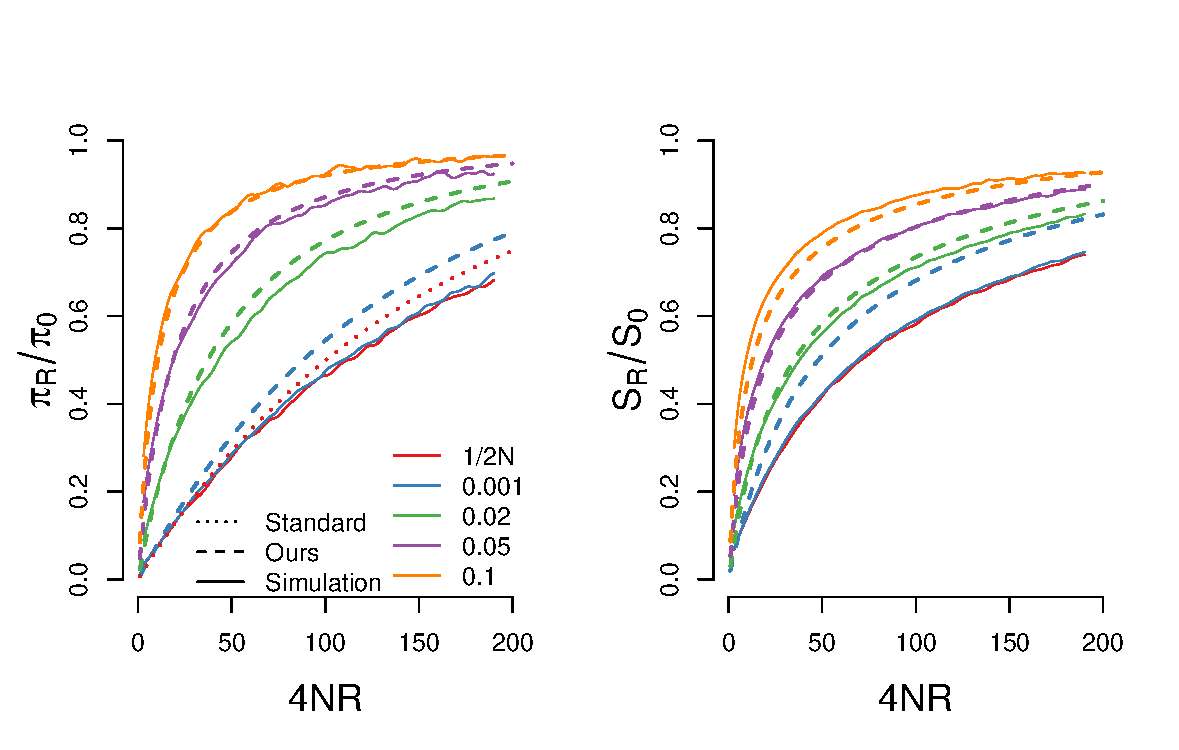
\includegraphics[width = \textwidth]{../Paper_Figures/pi_and_S_density.pdf} 
	\caption{A comparison of our approximations for the reduction in pairwise diveristy (A) and the number of segregating sites (B) for a sweep with $s=0.05$ and $N=10000$ starting from a variety of different frequencies. The approximations are generally accurate so long as the sweep begins from a frequency greater than $5/2Ns$, which is in this case $0.005$.} \label{pi_plot}
\end{figure}


\paragraph{Reduction in Pairwise Diversity}

The expected reduction in pairwise diversity following a standing sweep relative to neutral expectation is given by the probability that at least one lineage in a sample of two manages to recombine off of the \textbf{B} background (during either the sweep phase or the standing phase) before the coalescent event during the standing phase
\begin{equation}
	\mathbb{E}\left(\frac{\pi_R}{\pi_0}\right) \approx \left(1-\frac{1}{1 + R_f} e^{-\frac{r}{s}ln\left(\frac{1}{f}\right)}  \right) \label{pi_reduc}
\end{equation}
(Figure \ref{pi_plot}).
Given the exponential form of $P_{NR}$, and the fact that $\frac{1}{1+R_f}$ can be approximated as $e^{-R_f}$ for small values of $R_f$, we can further approximate \eqref{pi_reduc} as $1- e^{-r\bigl(\frac{ln\left(\frac{1}{f}\right)}{s} + 4Nf(1-f)\bigr)}$. Recalling that the reduction in diversity for a classic hard sweep with strong selection can be approximated as $1- e^{-r\bigl(\frac{log\left(2N_e \hat{s}\right)}{\hat{s}}\bigr)}$ \citep{Durrett:2004fl,Pennings2006}, it is tempting to suppose that there may exist a choice of $\hat{s}$, an ``effective'' selection coefficient, for which the classic hard sweep model produces a reduction in diversity over the same scale as the standing sweep model. While it is simple to set the the terms in the exponentials equal to one another and solve for the appropriate value of $\hat{s}$ (see Appendix), it turns out that for all choices of $N_e$, $s$, and $f$ for which our model applies, $\hat{s} \approx \frac{1}{2N_e}$. In other words, the reduction in diversity caused by a sweep from standing variation cannot be caused by a hard sweep in which standard strong selection approximations apply. No doubt there is a choice of selection coefficient under which a weakly selected allele will produce a similar reduction in diversity, but there are no adequate approximations available under this model, and we do not pursue the necessary simulation studies here.

\paragraph{Number of Segregating Sites}
We can also use our approximation to calculate the total time in the genealogy at a given distance from the selected site, which allows us to calculate the expected number of segregating sites. Conditional on $m$ independent lineages escaping the sweep, the expected total time in the genealogy is $2N \sum_{j=1}^{m-1} 1/j$, the standard result for a neutral coalescent with $m$ lineages \citep{Watterson:1975ur}. For a moment conditioning on no recombination during the sweep phase, the probability that $k$ independent lineages escape during the standing phase, given that there are at least 2 (otherwise all coalescence occurs on the $\textbf{B}$ background and $T_{TOT} \approx 0$) is 
\begin{equation}
	p_{ESF}\left(k \mid R_f , n , k > 1\right) = \frac{p_{ESF}\left(k \mid R_f , n \right)}{1 - p_{ESF}\left(1 \mid R_f , n \right)}.
\end{equation}
Conditional on no recombination during the sweep phase, the expected time in the genealogy is
\begin{equation}
	\mathbb{E}\left(T_{TOT} \mid i = n \right)  \approx 2N \sum_{k=2}^n p_{ESF}(k\mid R_f,n, k>1)   \sum_{j=1}^{k+n-i-1} 1/j.
\end{equation}

When we allow for all possible numbers of singleton recombinants during the sweep phase, the expected total time in the genealogy is
\begin{equation}
	\begin{aligned}
		\mathbb{E}(T_{TOT})  	&\approx 2N \biggl( P_{NR}(i=n\mid  n)  \sum_{k=2}^n p_{ESF}(k\mid R_f,n , k > 1)   \sum_{j=1}^{k+n-i-1} 1/j \\
							&+ \sum_{i=0}^{n-1} P_{NR} ( i \mid n) \sum_{k=0}^i p_{ESF}(k\mid R_f,n)   \sum_{j=1}^{k+n-i-1} 1/j\biggr)
	\end{aligned}
\end{equation}
(note that we have taken $p_{ESF}\left(0 \mid R_f,0\right)=1$, and $p_{ESF}\left(0 \mid R_f,i\right)=0\ \forall\ i > 0$; whereas it is typically impossible to obtain a sample with zero alleles, in our case we must define these probabilities to accommodate the case in which all $n$ lineages recombine out during the sweep phase)
and the expected number of segregating sites can be found by multiplying this quantity by the mutation rate (Figure \ref{pi_plot}).

\paragraph{The Frequency Spectrum} We can also use our approximation to obtain an expression for the full frequency spectrum at sites surrounding a sweep from standing variation. To break the problem into approachable components, we first consider the frequency spectrum of an allele that is polymorphic within the set of lineages which do not recombine during the sweep (ignoring it's frequency in the sweep phase recombinants), and we condition on a fixed number $k$ recombinant families from the standing phase. Borrowing from \cite{Pennings2006} (equation 14 of their paper), if we condition on $j$ out of these $k$ recombinant lineages carrying a derived allele, then we can obtain the probability that $l$ of the $i$ sampled lineages carry the derived allele by summing over all possible partitions of the $i$ lineages into $k$ families such that the $j$ recombinant ancestors carrying the derived mutation have exactly $l$ descendants in the present day
\begin{align}
p_{anc}(l \mid j, ~k,~i) 	&= \sum_{\substack{i_1+\cdots +i_j=l \\i_{j+1}+\cdots + i_k=n-l}} p(\{i_1,\dots,i_k\} \mid k, n) \notag \\
					&= \frac{ {n \choose l} }{ {k \choose j} }\frac{ S(l,j)  S(n-l,k-j)  }{ S(n,k) } \label{ESF_gives_freq_spec}
\end{align}

Next, we write $q\left(j \mid k\right)$ to denote the number of polymorphic mutations that were present $j$ times among the $k$ ancestral lineages which escape the standing phase. For our purposes, we will assume this follows the standard neutral coalescent expectation 
\begin{equation}
	q(j \mid k) = 	\begin{cases}
					\frac{\theta}{j}, 	& k \geq 2 \\
					0,			& \text{otherwise}
				\end{cases}
\end{equation}
although an empirical frequency spectrum measured from genome-wide data, as in \cite{Nielsen:2005bla}, could also be used. The expected number of derived alleles that are present in $l$ out of $i$ sampled lineages, conditional on there having been $k$ recombinant families, is then 
\begin{equation}
	p_{anc}(l \mid k, i ) = \sum_{j=1}^{k-1} p(l \mid j,~k, ~i)q(j\mid k).
\end{equation}	
Summing over the distribution of $k$ given by \eqref{ESF1}, we obtain an expression for the frequency spectrum within the set of $i$ lineages which do not recombine during the sweep as
\begin{equation}
	p(l \mid i) =  \sum_{k=2}^{n}  p_{ESF}(k \mid R_f,i,k>1)  \sum_{j=1}^{k-1} q(j\mid k) p(l \mid j,~k, ~i) \label{no-sweep-rec-freq-spec}
\end{equation}
This expression is essentially identical to the one presented in equation 15 of \cite{Pennings2006}. The only difference is that the Ewens clustering parameter in their model is given by the beneficial mutation rate, and \gc{holds only for sites fully linked to the selected loci}, whereas in our model it is a linear function of the genetic distance from the selected site. In our model, this approximation is highly accurate for loci that are distant from the focal site, but breaks down for loci that are tightly linked. The reason for this is that very near the focal site, it is actually very unlikely that there have been any recombination events at all, and so while polymorphism is rare, when it is present it is likely to have arisen due to new mutations on the genealogy of the $\textbf{B}$ allele (in which case their distribution is that of the standard neutral frequency spectrum), rather than ancestrally. While a full accounting for the contribution of new mutations in regions where there has been at least one recombination event is beyond our scope, we can develop an \textit{ad hoc} approximation by assuming that mutations are new if there have not been any recombination events, and are old if there has been at least one recombination (see Appendix). This approximation is quite accurate, especially when the focal allele is at low frequency (Figure \ref{freq_spec}).

When we allow for recombination during the sweep, the expression becomes more complex, as we must take into account the fact that a mutation may be polymorphic after the sweep even if it is either absent or fixed in the set of lineages which hitchhike. Nonetheless, we obtain an expression for the frequency spectrum of ancestral polymorphism as
\begin{equation}
		p(l \mid n ) = \sum_{i=0}^n P_{NR}(i\mid  n) \sum_{k=1}^{i} p_{ESF}(k \mid R_f,n-i) \sum_{j=1}^{\text{min}\left(k+n-i-1,\ell\right)} q(j\mid k+n-i) \sum_{g = \text{max} \left( j - k , 0 \right) }^{\text{min} \left( j , \ell , \left(n-i\right) \right)} H(g \mid j,k,n-i) p(\ell-g \mid j-g,k,i) \label{rearrange-anc-freq-spec}
\end{equation}
where
\begin{equation}
	H(g \mid j,k,n-i) = \frac{{n-i \choose g}{k \choose j - g}}{{k + n - i \choose j}}
\end{equation}
gives the probability that $g$ out of a total of $j$ derived alleles which existed before the sweep are found on singleton recombinants created during the sweep, given that there are $n-i$ singletons, and $k$ recombinant families created during the standing phase. 

In words, $n-i$ lineages recombine out during the selected phase, while the remaining $i$ lineages are partitioned into $k$ families at frequencies $\{i_1,\dots,i_k\}$ due to recombination and coalescence in the standing phase. Out of the $n-i$ singleton lineages, $g$ of them carry the derived allele, while the remaining $j-g$ copies of the derived allele give rise to $l-g$ derived alleles due to coalescence during the standing phase, and we take the sum over all possible combinations of these values which result in a final frequency of  $\frac{l}{n}$ in the present day sample.

Once again, this expression is accurate far from the selected site, but in error at closely linked sites due to the contribution of new mutations. Again, we can develop an \textit{ad hoc} approximation by allowing for new mutations during the sweep phase on any lineage that does not recombine during that phase, and on the $i$ lineages that reach the standing phase, provided there are no recombination events during that phase (see Appendix and Figure \ref{freq_spec}). New mutations during the standing phase are ignored once there has been at least one recombination event during that phase. This approximation is quite accurate at all distances (especially when the sweep comes from relatively low frequency), appropriately capturing the uptick in singleton frequency close to the selected site due to new mutations occurring during the sweep phase. Inaccuracies for sweeps coming from higher frequencies arise in large part from the fact that the genealogy of the \textbf{B} alleles is large enough that there is still a substantial contribution of new mutations from the standing phase even when there have been multiple recombination events during that phase.

\begin{figure}
	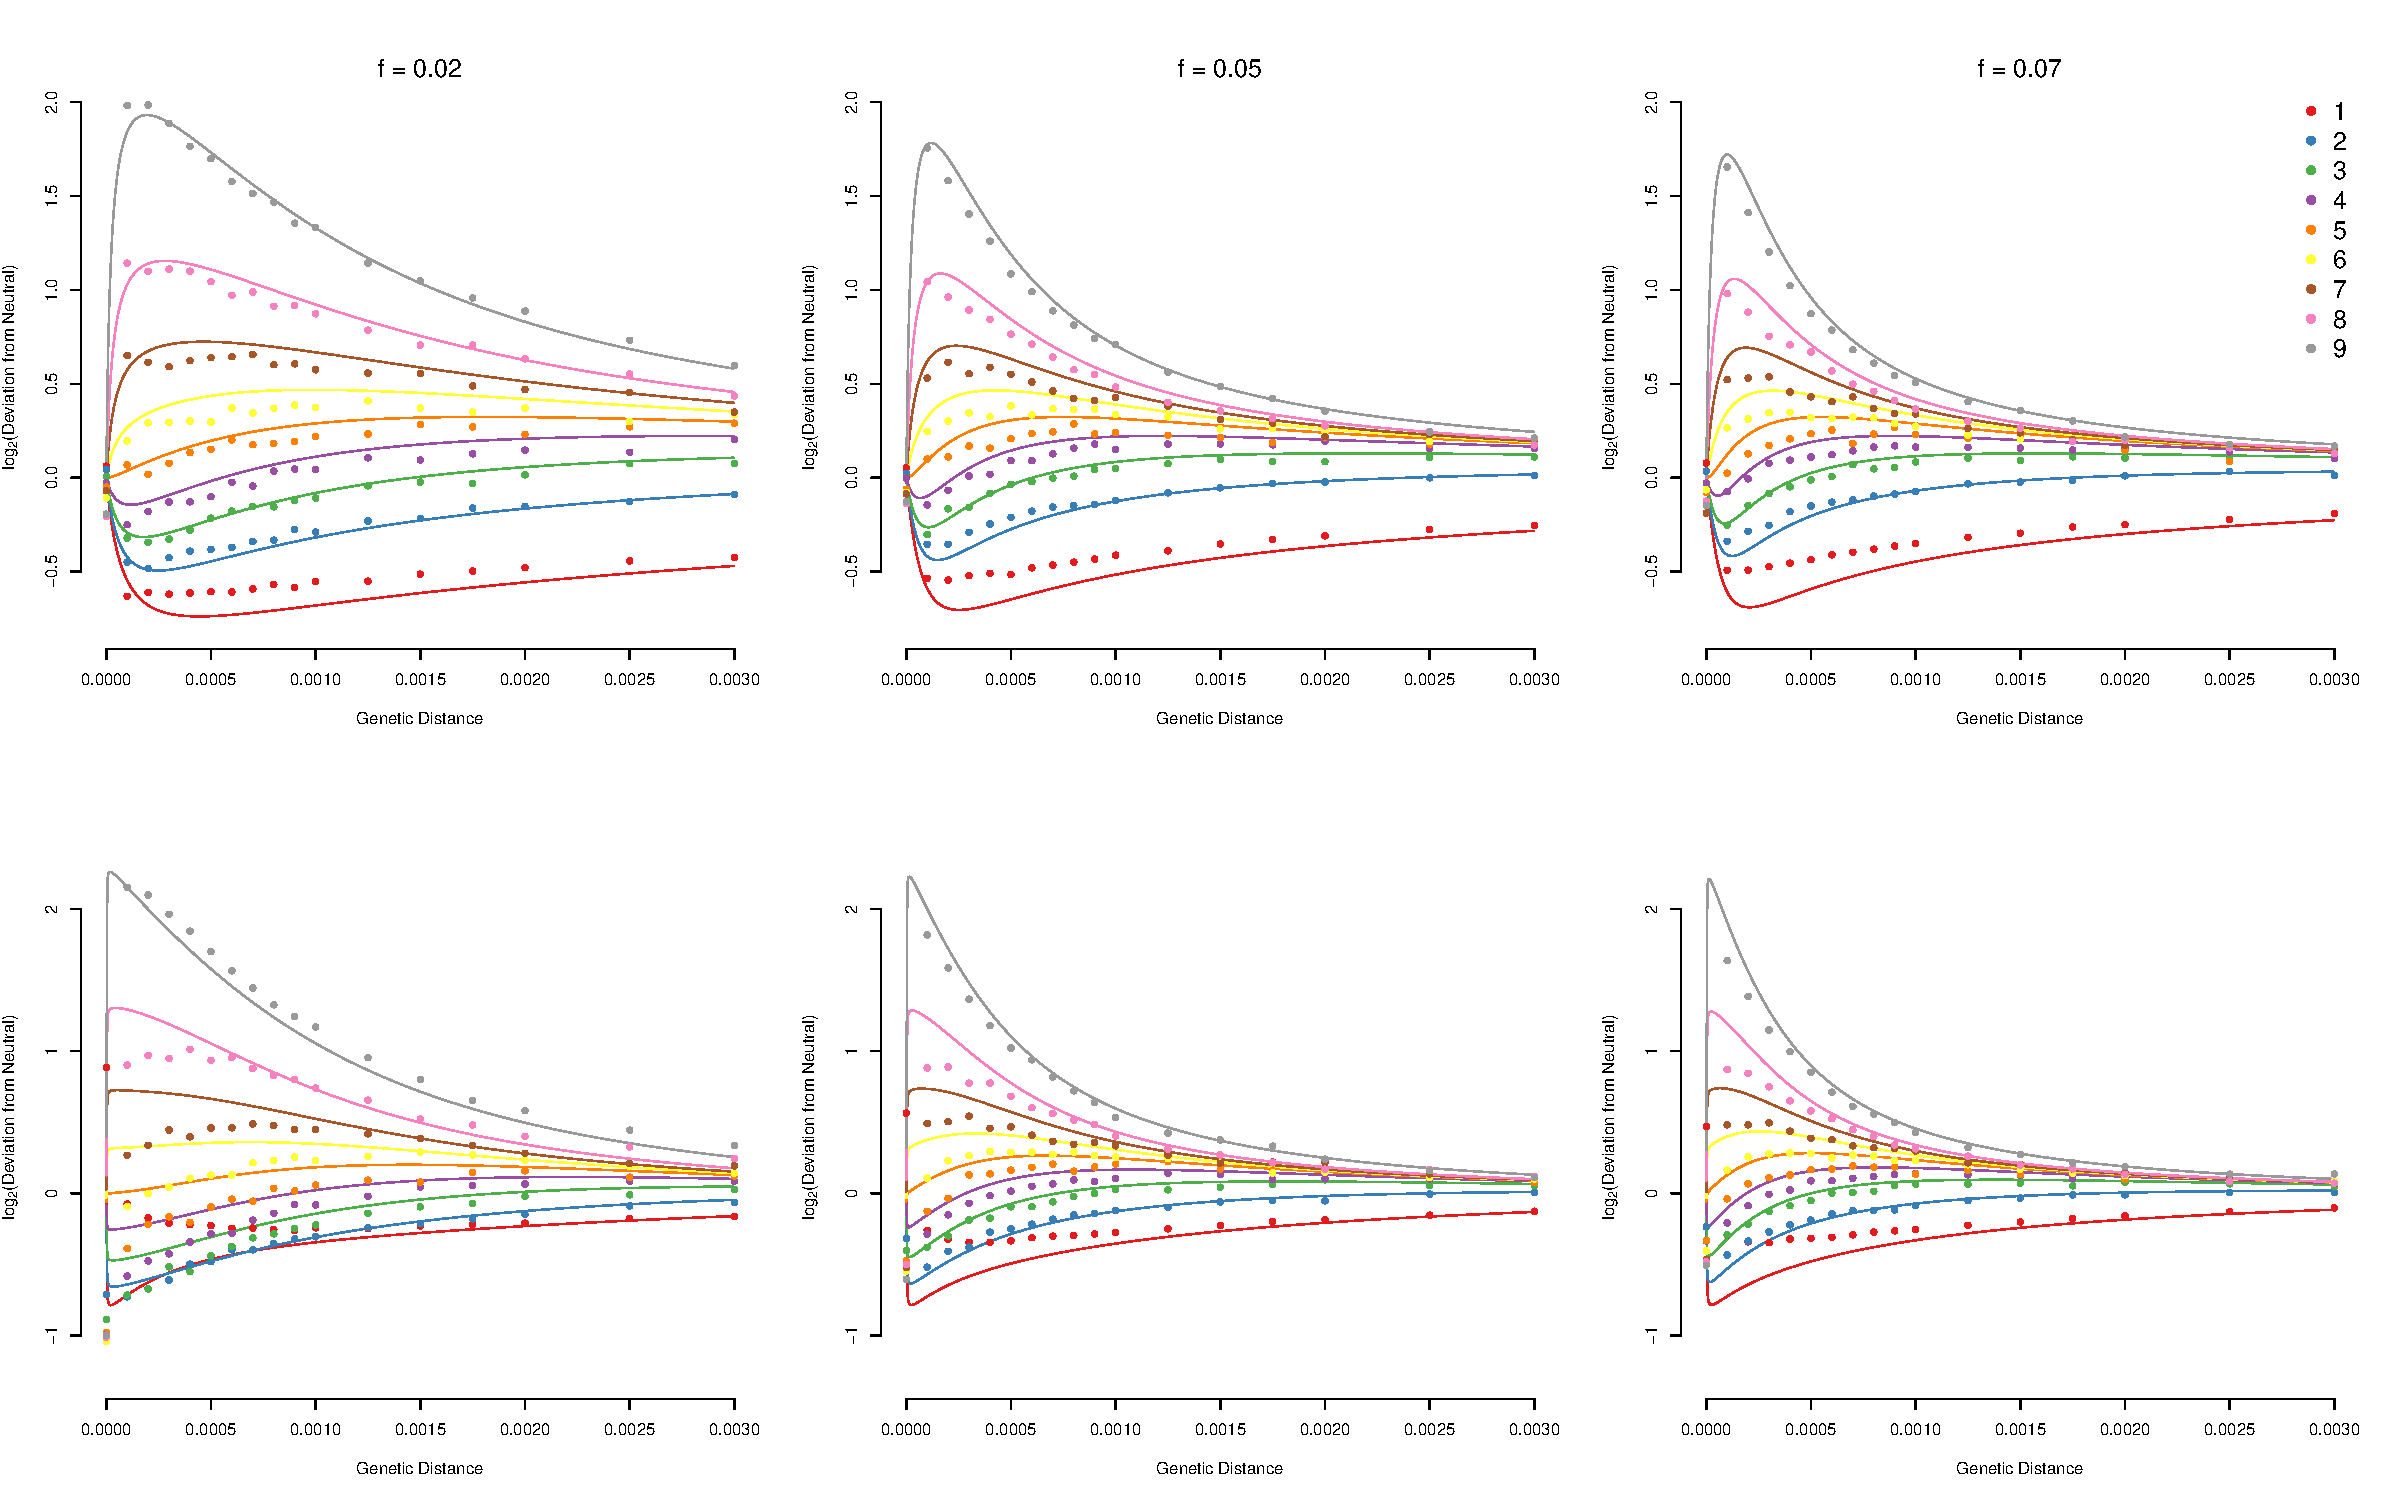
\includegraphics[width = \textwidth]{../Paper_Figures/freq_spec_nosweep_logfold_sixpanel_020507.pdf}
	\caption{The frequency spectrum, in a sample of n = 10, for a neutral allele sampled on the background of the beneficial allele either immediately before it sweeps (A,B,C) or immediately after fixation (D,E,F). Results are shown as the log ratio of the normalized frequency relative to its expectation under the standard neutral coalescent.} \label{freq_spec}
\end{figure}

\subsection*{Patterns of Haplotype Variation and Routes to Inference}

We continue with our infinitely-many haplotypes perspective, in which we imagine that every piece of DNA present in the sample taken at fixation can be labelled/colored according to which chromosome in the ancestral, pre-sweep population it traces its ancestry to. Under this convention, right at the selected site, all chromosomes descending from either a hard sweep or a standing sweep will be of the same ``color'', due to their shared common ancestry, while for multiple mutation soft sweeps each set of chromosomes tracing to a different mutational origin of the beneficial allele will be of a different color. For all kinds of sweeps, the number of distinctly colored haplotypes increases with distance from the selected site due to recombination events off of the \textbf{B} background, each of which subdivides a single class of haplotypically equivalent sequences into two subclasses (e.g. see Figure \ref{cartoon_fig_2}).

Unfortunately, explicit analytical expressions for these haplotype partition transitions are unavailable under any sweep model, and ours is no exception. Nonetheless, we gain some insight from a simple description of the process, and this descriptions motivates some further simulations.

Recall that $\tau_{f}$, the duration of the sweep, is of order $1/s$, while the time from the beginning of the standing phase back to the common ancestor of the beneficial alleles is approximately $4N_e f$. Therefore, if $4N_e s f \ll 1$ (i.e. selection is weak, or the mutation is still quite rare when selection switches on), singleton recombination events during the sweep phase erase any signal of the fact that the allele was previously standing, and the eventual pattern is very similar to that of a hard sweep.

The alternate extreme of $4N_e s f \gg 1$ occurs when selection is strong or the mutation was segregating at a relatively high frequency prior to the onset of selection. In this parameter regime, the sweep phase occurs fast enough that recombination events from this period tend to be far away from the selected site, and the structure of the haplotype partition is dominated by events in the standing phase. Below, we consider constructing the haplotype partition as a process along the sequence in the limit $4N_e s f \rightarrow \infty$, ignoring the sweep phase.

If the total time in the coalescent tree in the neutral phase at the selected site is $T_{stand}$, then the distance to the first recombination is $\sim \exp \left( r_{BP}\left(1-f\right) T_{stand} \right)$. Using the standard approximation for the total time in the tree, the expected length scale over which a single haplotype should persist away from the selected site is $\approx 1/( 2 N_e r_{BP}f\left(1-f\right) log(n-1))$ (and twice this distance if we consider both sides of the sweep). This recombination partitions the haplotypes according to the neutral frequency spectrum (e.g. the green recombinant moving to the left in Figure \ref{cartoon_fig_2}C). Moving down the sequence we then generate the next distance to a recombination, again from $\sim \exp \left( r_{BP}\left(1-f\right) T_{stand} \right)$. We again uniformly simulate a position on the tree for this new recombination, however, this time only a recombination on some of the branches would result in a new haplotype being introduced into the sample (e.g. the red recombinant in Figure \ref{cartoon_fig_2}B is responsible for the second transition in the haplotype partition scheme in Figure \ref{cartoon_fig_2}C). If the recombination falls in a place that doesn't alter the configuration we ignore it and simulate another distance from this new position. Otherwise, we keep the recombination event and split the sample configuration again. (For example, the orange recombinant in Figure \ref{cartoon_fig_2}C does not alter the status of identity by descent relationships with respect to the sweep, and therefore does not result in an increase in the number of haplotypes under our convention. It may, however, result in a change in the practical ability to distinguish the those two sequences as belonging to a distinct haplotype from the others, due to rearrangements in the ancestral genealogy which affect the probability that there will be observable ancestral polymorphism distinct to those two sequences.) We iterate this procedure moving away from the selected site, generating exponential distances to the next recombination, placing the recombination down, updating the configuration if needed, until we reach the point that every colored haplotype is a singleton. We then repeat this procedure on the other side of the selected site using the same underlying genealogy.

An equivalent way to describe this process is to simulate distances to the next recombination that alters the configuration, given the tree and the previous recombinations. To do this we consider the total time in the tree where a recombination would alter the configuration. Numbering these recombinations out from the selected site,  we start at the selected site $i=0$, with $T_0 = T_{stand}$ and generate a distance to the first recombination $\sim \exp(r_{BP}\left(1-f\right) T_0)$. We place the recombination on the tree, then prune the tree of branches where no further change in sample configuration could result in a new colored haplotype. We then set $T_i$ to the total time in these pruned subtrees, place the next recombination uniformly on the pruned branches at an $\sim \exp(r_{BP}\left(1-f\right) T_i)$ distance and carry on this process till we have pruned the entire tree such that all lineages reach their own unique recombination event before coalescing with any other lineage.

To simulate a sequence that includes the effect of the sweep phase, we simply generate an $\sim \exp\left(\frac{r_{BP}}{s}ln\left(\frac{1}{f}\right)\right)$ distance for each chromosome independently and superimpose this recombination process on top of the one described above. Between the selected site and this sweep phase event, each sequence's haplotype identity is defined by the process described above. Beyond, it is a singleton.

\paragraph{Routes to Inference}
As discussed above, marginally at a given site the partitioning of haplotypes (integrating out the unobserved genealogy) is given by the ESF. It is unclear to us how to couple together the partitioning at two sites in an analytically tractable way. For example, efficient ways of computing 
\begin{equation}
	P\left(\{i_1,i_2,\dots,i_k,\dots,i_{k+j}\} \text{ at position } r_2 \mid \{i_1,i_2,\dots,i_k\} \text{ at position } r_1 \right) \label{conditional-density}
\end{equation}
and related expressions, in combination with some of the machinery we use above for our frequency spectrum calculations could in principle be used to take a product of approximate conditional (PAC) likelihoods approach to inference under different sweep models. Of course, such computations could be done via brute force numerical integration over all possible genealogies, but this is unfeasible for any sample size large enough to be useful. One would need to be able to calculate such quantities under multiple different sweep models in order to deploy them, and so this would require further development under all three models. A more direct (and perhaps accurate) route to inference may actually be to build upon recent developments in coalescent HMMs \citep{Li2011,Paul:2011gv,Sheehan:2013ib,Rasmussen:2014gj} and explicitly model the effect of selective sweeps on the ancestral recombination graph. Our model suggests a way to accomplish this effectively for sweeps from standing variation, and recent work on both hard and soft sweeps \citep{Barton1998,Durrett:2004fl,Durrett:2005fr,Schweinsberg:2005eh,Etheridge:2006fk,Hermisson2008,Messer:2012ie} provide a route to doing so under these models. A third approach, which we explore below, is to continue along the lines of popular sweep finding approaches implemented to date, and define summary statistics which can effectively distinguish between different models. Nonetheless, while both of these approaches seem more likely to be fruitful than the PAC approach described above, expressions like \eqref{conditional-density} would represent significant progress in relating the infinite alleles and infinite sites models, and given the general interest in the ESF motivated by exchangeable partitions and clustering algorithms, are likely of wider interest.
 
\subsubsection*{Observed haplotype frequency spectum}

To this point, our discussions of haplotype variation have focused on haplotypes defined via identity-by-descent, which cannot be observed directly. It is useful to consider how the understanding gained here can be leveraged to improve our ability to identify standing sweeps. To do this we turn to the ordered haplotype frequency spectrum.


%One possible approach is to modify the prior in recently developed algorithms for sampling from the ancestral recombination graph \citep[e.g. ARGweaver,][]{Rasmussen:2014gj} to approximate the genealogical distortions expected under different sweep scenarios. This approach seems likely to be fruitful, but lies beyond the scope of this paper.

%An alternate possibility which seems potentially fruitful is to identify a set of summary statistics which can jointly distinguish swept regions from non-swept regions, as well as distinguish among different kinds of sweeps. 

For a window of size $L$, we define the the ordered haplotype frequency spectrum (OHFS) as $\mathcal{H}_L = \{h_1,h_2,\dots,h_{H_{L}}\}$, where $h_p$ gives the sample frequency of the $p^{th}$ most common haplotype and there are a total of $H_{L}$ distinct haplotypes within the window. Coarse summaries of the OHFS have been a popular vehicle for sweep-finding methods \cite[e.g. EHH, iHS and H12:][]{Sabeti:2002ge,Voight:2006go,Garud:2015jy,Garud:2015fe}. We focus on identifying which aspects of the OHFS should be most informative about the size, as well as the shape of the genealogy at the focal site.

Specifically, we conducted coalescent simulations with a sample size of $n=100$ chromosomes under four different models of sequence evolution (hard sweeps, standing sweeps from $f=0.05$, soft sweeps conditional on three origins of the beneficial mutation, and neutral), with all sweep simulations set to $s=0.01$. For the standing sweeps, this corresponds to $4Nsf = 20$, and thus to a scenario where the standing phase has a slightly stronger, but not overwhelming, impact on the final patterns of haplotype diversity.

One simple prediction on the basis of our analytical investigation above is that, because the genealogy under a standing sweep is generally larger than that under a hard sweep, recombination events out of the sweep should accumulate more quickly along the sequence and therefore the total number of haplotypes in a window of a given size should be larger for a standing sweep than for a hard sweep. In Figure \ref{hap-exist-probs} we show from simulations $P\left(H_L^{stand} \geq i \right)/P\left(H_L^{hard} \geq i \right)$ over a range of $L$ for one sided windows extending away from the selected site. As expected, we see that the number of haplotypes increases more quickly with distance from the selected site for a standing sweep than for a hard sweep. Unfortunately, as we alluded to above, this signal is largely confounded by the fact that one can also obtain a similarly rapid increase in the number of haplotypes from a hard sweep with a slightly weaker selection coefficient.

\begin{figure}
		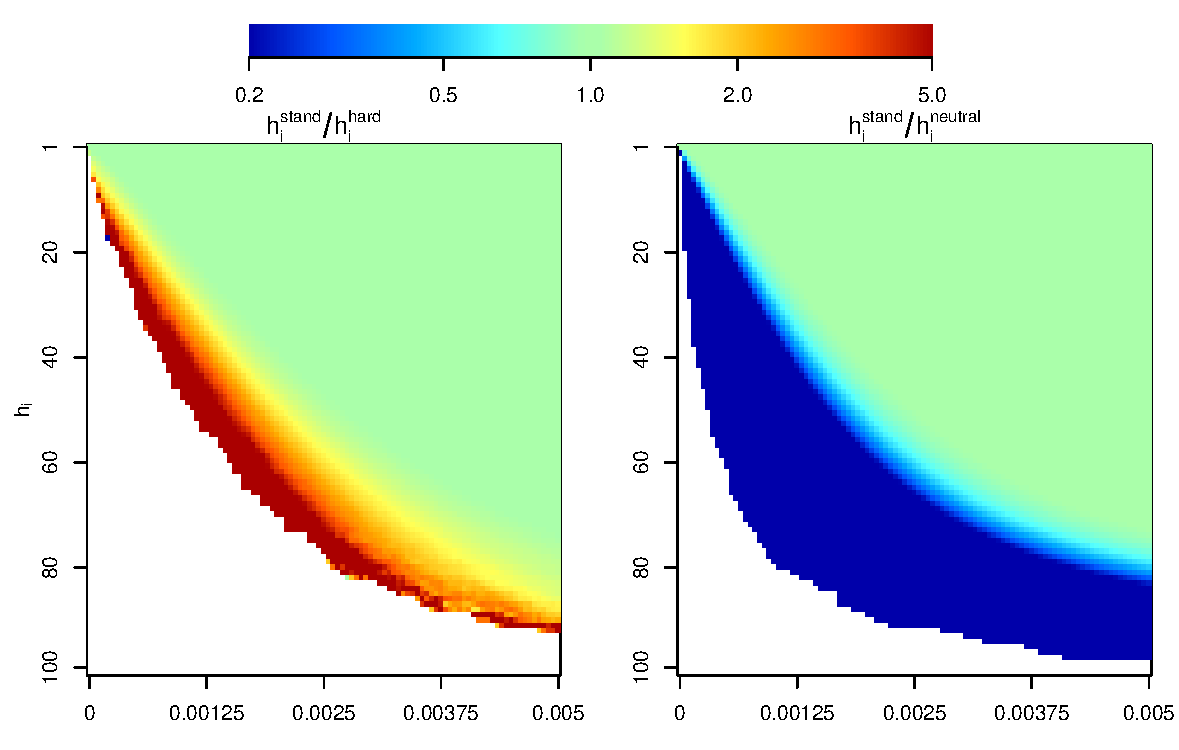
\includegraphics[width = \textwidth]{../Paper_Figures/HapFreqsExistProb.pdf}
	\caption{The ratio of the probability that there are at least $i$ haplotypes in a one sided window extending away from the selected site for the standing sweep model relative to the hard sweep model (A) and the neutral model (B).} \label{hap-exist-probs}
\end{figure}

Alternately, we may hope to use to OHFS to obtain information about the shape of the genealogy at the focal site, which should hopefully be less confounded by a change in selection coefficient. This information is found in differences in the relative frequencies of certain haplotypes between the different models, rather than in the total number of haplotypes. Specifically, if there are multiple haplotypes present close to the selected site,  they should be more common under the sweeps from standing variation model than the full sweep model. In other words, there should be a window near the selected site where $\mathbb{E}[h_i^{stand} \mid h_i^{stand} > 0] > \mathbb{E}[h_i^{hard} \mid h_i^{hard} > 0]$ for $1 < i \ll n$, owing to recombinations occurring on internal branches of the genealogy from the standing phase. 

In Figure \ref{hap-freq-ratios}, we show $\mathbb{E}[h_i^{M1} \mid h_i^{M1} > 0]/\mathbb{E}[h_i^{M2} \mid h_i^{M2} > 0]$ where $M1$ and $M2$ denote different models of sequence evolution (i.e. standing, hard, or soft sweep or neutral). In particular, we wish to draw attention to the fact that, similar to the multiple mutation model, most of the useful information within the OHFS for distinguishing standing sweeps from hard sweeps lies within a small window near the selected site, and comes in the form of a decrease in the relative frequency of the core haplotype, and corresponding overabundance of the next few most common haplotypes. In contrast to the multiple mutation case, the enrichment of moderate frequency haplotypes for the standing case is relatively subtle, and beyond moderate recombination distances, there is little information to distinguish a standing sweep from a hard sweep. We also observe that, contrary to multiple mutation soft sweep model, far away from the selected site, standing sweeps resemble hard sweeps across the majority of the OHFS. This is in line with expectations from our results above, in that close to the selected site the haplotype partition is dominated by events occurring during the standing phase, while far from the selected site it is dominated by events occurring during the sweep phase.

On the basis of these simulation results, we suspect that future methods for identifying and distinguishing different varieties of sweeps will see benefits from incorporating haplotypic information over a range of window sizes surrounding the focal site, and from pushing deeper into the haplotype frequency spectrum, particularly when large samples are available. 

\begin{figure}
	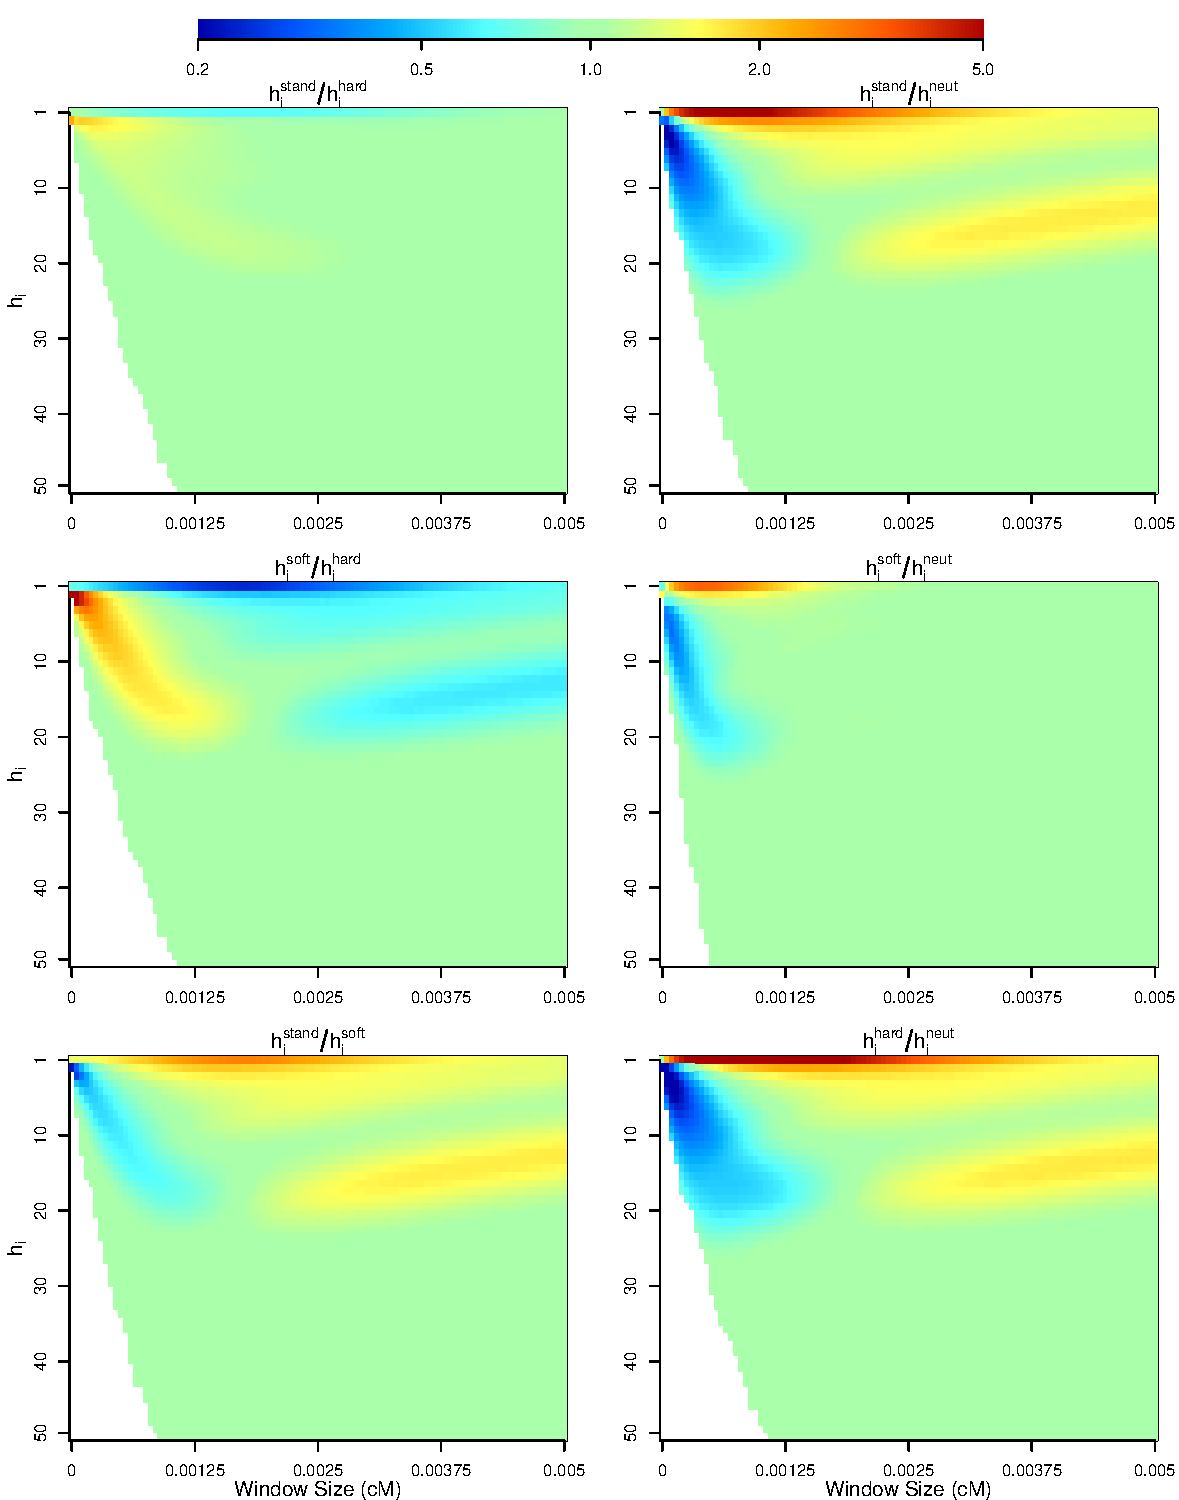
\includegraphics[width = 0.8\textwidth]{../Paper_Figures/HapFreqRatiosCondExist.pdf} 
	\caption{caption goes here} \label{hap-freq-ratios}
\end{figure}

%
%\gc{points to hit}
%
%Are s and f distinguishable or both inferable.
%--Weak selection maybe everyone recoms out
%--Large f maybe no signal of sweep?
%--What fraction of the singleton recombinants come from selected vs stand phases?
%--Do you get to see the singleton recombinants from the sweep. Total coalescent time in sweep phase vs total time in standing phase?
%
%Comparison to multiple mutations. 
%--What makes the two cases distinguishable
%--Code up? Pennings and Hermisson.
%
%
%Time since to sweep. 
%--does this mess things up?
%--scale of recombination and coalescence leading up to sweep.
%--Maybe just have this discussion.

\section*{Discussion}

An accurate portrait of the patterns of sequence diversity expected in the presence of recent or ongoing positive selection has proven to be vital for the identification of adaptive loci. Recent theoretical and empirical work has drawn attention to the fact that adaptation from standing variation may be relatively common, and that patterns of sequence variation produced in such scenarios may differ markedly from those produced under the classical hard sweep model. In this paper, we've focused on developing a tractable model of strong positive selection on a single mutation which was previously segregating (or balanced) at low frequency. We have shown that many aspects of the pre-sweep standing phase of the mutation's history on post-hitchhiking patterns variation can be approximated via an application of the Ewens Sampling Formula. This provides a way to build intution for the process and obtain various analytical approximations for patterns of variation following a sweep from standing variation. 

Our results can be understood within the context of a number of recent approximations for different sweep phenomena, which divide the sweep into distinct phases \citep[see e.g.][]{Barton1998,Etheridge:2006fk}. Because rates of coalescence and recombination vary across these phases, different sections of the sequence surrounding a sweep will convey information about different phases, with sites distant from the selected locus generally conveying information about the late stages of the sweep, and sites close to the selected locus conveying information about the early stages of the sweep. In our model, the late phase corresponds largely to what we've called the sweep phase, while the early phase corresponds to our standing phase. In general, the major differences between different sweep phenomena occur during the earliest phases, and thus the information to distinguish them is found near to the selected site, while extra information about the strength of the sweep can be found at sites that are more distant.

It is worth noting however that all of our results are obtained for populations with equilibrium demographics. If population size is variable, particularly over the course of the standing phase, then the ESF fails to accurately describe recombinations during this phase, just as it fails to accurately describe the infinite alleles model with non-equilibrium demographics. Inference methods based on our analytical calculations would likely be inaccurate in these situations \citep{Bank:2014hx}. Nonetheless, the general insight remains that, holding demography equal, sweeps from standing variation will generate genealogies with longer internal branches than classic hard sweeps, and will therefore be characterized by more intermediate frequency haplotypes. 

Although we do not pursue it, essentially all of our results also likely apply to fully recessive sweeps from \textit{de novo} mutation. This is because a recessive beneficial mutation is effectively neutral until it reaches sufficient frequency for homozygotes to be formed at appreciable enough rates to feel the effects of selection. The result is that recessive sweeps should be fairly well approximated by setting $f = \frac{1}{\sqrt{2Ns}}$ in our model for the standing phase and taking the value of $P_{NR}$ for the latter phase to be
\begin{equation}
	\exp\left(-r \int_{\frac{1}{\sqrt{2Ns}}}^1\left(1-X\right)g\left(X\right)\mathrm{d}X\right)
\end{equation}
where $g\left(X\right)$ is the Green's function for a recessive allele under positive selection. This conclusion is foreseen by \cite{Ewing:2010bg}, who suggested just this sort of approximation for the reduction in diversity following a recessive sweep. The result is that it is likely to be fundamentally impossible to distinguish between a sweep from previously neutral or balanced standing variation and a recessive sweep without additional biological information about dominance relationships at the locus of interest.

Unfortunately, our work largely confirms the intuition and existing results indicating that standing sweeps are likely to be rather difficult to identify, and characterize, on the basis of genetic data from a single population time-point, and when they can be identified, they will be difficult to distinguish from classic hard sweeps \citep{Peter:2012ht}. This can be understood from first principles by recognizing that the identification of a standing sweep amounts to recognizing that a particular region of the genome effectively experienced a reduction in effective population size by a factor of $f$, followed by a period of rapid growth back up to the $N_e$ experienced by the bulk of the genome. This task is made difficult by the fact that one has effectively only a single genealogy with which to make this inference, rather imperfect information about its shape and size, and that it shares features both with genealogies expected under a classic hard sweep and under neutrality.

As a result, we suspect that efforts to detect selection from standing variation will continue to be most effective when additional data is available from populations where the allele was not favored or failed to spread for some other reason \citep{Innan:2008ii,Chen:2010ic,Roesti:2014gp}. If we have good evidence that the allele has spread rapidly, e.g. if the populations are very closely related, then evidence that it is a sweep from standing variation could be gained from demonstrating that the genomic width of the sweep was much smaller than expected given how quickly it would have to have transited through the population. Ancient DNA is also likely to be of value, as we may similarly be able to identify alleles that were at low frequency too recently in the past given observed present day patterns of genetic variation.


\section*{Simulation Details}

In order to check our analytical results, we wrote a program to simulate allele frequency trajectories under our model, and then ran either custom written structured coalescent simulations (Figures \ref{Prob_hap_distribution}, \ref{n_2_supp_plot}, \ref{mean_coal_times_supp_plot} and \ref{coeff_var_coal_times_supp_plot}) or handed these trajectories to \textit{mssel} in order to generate sequence data (Figures \ref{pi_plot}, \ref{freq_spec}, \ref{hap-exist-probs} and \ref{hap-freq-ratios}).

\subsection*{Frequency Trajectories}
We simulate frequency trajectories under a similar discretized approximation to the diffusion as that used by \cite{Przeworski2005}. In order to simulate trajectories conditional on selection having begun when the allele was at frequency $f$, we set $X\left(0\right) = f$, and simulate allele frequency change forward in time according to
\begin{equation}
	X\left({t+1}\right) \sim N \left( \mu_S\left(X\left(t\right)\right)\Delta t , \sigma\left(X\left(t\right)\right)\Delta t \right)
\end{equation}
where
\begin{align}
	\mu_S\left(X\left(t\right)\right) &= \frac{2NsX\left(t\right)\left(1-X\left(t\right)\right)}{\textrm{tanh}\left(2NsX\left(t\right)\right)} \\
	\sigma\left(X\left(t\right)\right) &= X\left(t\right)\left(1-X\left(t\right)\right)
\end{align}
and we take $\Delta t = \frac{1}{2N}$ so that one time step is equivalent to the duration of one generation in the discrete time Wright-Fisher model, and we have conditioned on the eventual fixation of the allele. To simulate the neutral portion of the frequency trajectory prior to the onset of selection, conditional on the allele having been derived, we take advantage of the time reversibility property of the diffusion process, which dictates that the distribution on the prior history of an allele conditional on being derived and being found at frequency $f$ is the same as the future trajectory of an allele that is at frequency $f$ and destined to be lost from the population. This allows us to simulate from
\begin{equation}
	X\left(t-1\right) \sim N\left(\mu_N\left(X\left(t\right)\right) \Delta t, \sigma \left( X\left(t\right) \right)\Delta t\right)
\end{equation}
where
\begin{equation}
	\mu_N\left(X\left(t\right)\right) = - X\left(t\right).
\end{equation}
We simply then paste these two trajectories together to give a frequency trajectory that is conditioned on a sweep beginning when the allele is at frequency $f$ without any unnatural conditioning on the sweep beginning the \textit{first} time the allele reaches frequency $f$. For simulations intended to check our standing phase calculation independent of the sweep phase, we simply discard the sweep portion of the simulation and retain only the neutral trajectory.

\subsection*{Genealogy and Recombination Histories}

We simulate the genealogy backward in time at the locus of the beneficial allele by allowing a coalescent event to occur between two randomly chosen lineages in generation $t$ with probability $\frac{{n\left(t\right) \choose 2}}{2NX\left(t\right)}$, where $n\left(t\right)$ gives the number of lineages existing in generation $t$. Coalescent times obtained from these simulations are then used to generate Figures \ref{n_2_supp_plot}, \ref{mean_coal_times_supp_plot}, and \ref{coeff_var_coal_times_supp_plot}. We then simulate the history of recombination events which move lineages off of the beneficial background as follows:

We calculate the total time in the genealogy, $T$, and simulate an $\exp\left(-rT\right)$ distance to the first recombination event. A position on the tree (i.e. a branch and a specific generation for the event to occur in) is chosen uniformly at random. This event is accepted with probability $1-X\left(t_{rec}\right)$, where $t_{rec}$ gives the generation in which the event occurred, otherwise it is ignored. This process is repeated outward away from the focal site until the end of the sequence is reached, and the physical position along the sequence, the branch, and the generation of each recombination event is recorded.

We then generate haplotype identities (i.e. the colorings of Figure \ref{cartoon_fig_2}) as follows. We begin at the root of the tree, and assign each sequence to have the same identity over their entire length. We then move forward in time, from one recombination event to the next, and for each recombination event we assign the chromosomes which subtend it a unique new identity extending from the position where that event occurred out the end of the sequence, overwriting whatever identity previously existed there. We iterate this procedure all the way until the present day, at which point each position on a given chromosome will have an identity specified by the most recent recombination event which falls in between it and the focal site. These haplotype identities are what we use to generate Figure \ref{Prob_hap_distribution}.

\subsection*{Simulated Sequence Data}

To simulate sequence data, we simply hand the trajectories simulated as described above to the program \textit{mssel} \jb{reference?}. Whereas our simulations of haplotype identity above still represents a somewhat heuristic approximation to the true process, in that it ignores recombination events which do not result in transitions to the alternate background, these simulations of sequence data are exact under the structured coalescent with recombination for our model up the discretization of the diffusion process used for the selected allele. These simulations are used to generate Figures \ref{pi_plot}, \ref{freq_spec}, \ref{hap-exist-probs} and \ref{hap-freq-ratios}.

\paragraph{Code Availability:} All custom simulation code was written by JB in R and is provided in Supplementary File 1.
\section*{Appendix}

\subsection*{Incompatibility of Standing Sweep and Classic Strong Selection Models}

Consider the small $r$ approximation $\exp\left( -r \left(\frac{1}{s}ln\left(\frac{1}{f}\right) + 4Nf\left(1-f\right)\right) \right)$ for the probability of failing to recombine before coalescing under our standing sweep model, and $\exp\left( - \frac{r}{\hat{s}}ln\left(2N\hat{s}\right) \right)$ for the same probability under the hard sweep model. We can set these two expressions equal to one another and solve for $\hat{s}$, yielding
\begin{equation}
	\hat{s} = \frac{1}{2N_e} e^{-W\left(\frac{4N_e sf^2 - 4N_e s f  - ln \left( \frac{1}{f} \right)}{2N_es}\right)}
\end{equation}
where $W\left(z\right)$ is Lambert's W function. 

\subsection*{Inclusion of New Mutations in Frequency Spectrum}
In the main text, we defined $q(j \mid k)$ as the expected number of segregating mutations present on $j$ out of $k$ ancestral lineages. Here, we introduce a subscript $q_{anc}(j \mid k) = \frac{\theta}{j}$ and then define 
\begin{equation}
	q_{new}(l \mid k, i, n) =
	\begin{cases} 
		\frac{\theta f}{l}, 	& \text{if } i = n, k = 1 \\
		0, 				& \text{otherwise}.
	\end{cases}
\end{equation}
We can then give an improvement upon equation \eqref{no-sweep-rec-freq-spec} as
\begin{equation}
	p(l \mid i) =  \sum_{k=2}^{n}  p_{ESF}(k \mid R_f,i)  \sum_{j=1}^{k-1} \left(q_{anc}(j\mid k)p(l \mid j,~k, ~i)  + q_{new}(l \mid k,i,n) \right)
\end{equation}
and obtain the normalized version by dividing by their sum.

We can make an improvement upon equation \eqref{rearrange-anc-freq-spec} in a similar manner. We first redefine
\begin{equation}
	q_{new}(l \mid k, i, n) =
	\begin{cases} 
		\theta f + \mu n\frac{\tau_f}{2}, 	& \text{if } i = n, k = 1, l=1 \\
		\mu i\frac{\tau_f}{2},			& \text{if } i < n, k = 1, l =1 \\
		\frac{\theta f}{l},		& \text{if } i = n, k = 1, l > 1\\
		0, 				& \text{otherwise}.
	\end{cases}
\end{equation}
In other words, we allow new mutations to occur during the standing phase provided that there have been no recombination events during this phase, and we also allow new mutations during the sweep phase on all lineages which do not recombine during the sweep phase. Obtaining an improvement over equation \eqref{rearrange-anc-freq-spec} is then once again simply a matter of adding the term for new mutations into the previous expression

\begin{multline}
		p(l \mid n ) = \sum_{i=0}^n P_{NR}(i\mid  n) \sum_{k=1}^{i} p_{ESF}(k \mid R_f,n-i) \\
		\sum_{j=1}^{\text{min}\left(k+n-i-1,\ell\right)} \left(q_{new}(l \mid k,i,n) + q_{anc}(j\mid k+n-i)\sum_{g = \text{max} \left( j - k , 0 \right) }^{\text{min} \left( j , \ell , \left(n-i\right) \right)} H(g \mid j,k,n-i) p(\ell-g \mid j-g,k,i)\right) 
\end{multline}
%%%%%%%%%%%%%%%%%%%%%%%%%%%%
\section*{Acknowledgements}


\bibliographystyle{genetics}
\bibliography{library,morelibrary}

\section{Supplementary materials}

\setcounter{table}{0}
\renewcommand{\thetable}{S\arabic{table}}
\setcounter{figure}{0}
\renewcommand{\thefigure}{S\arabic{figure}}


\begin{figure}
	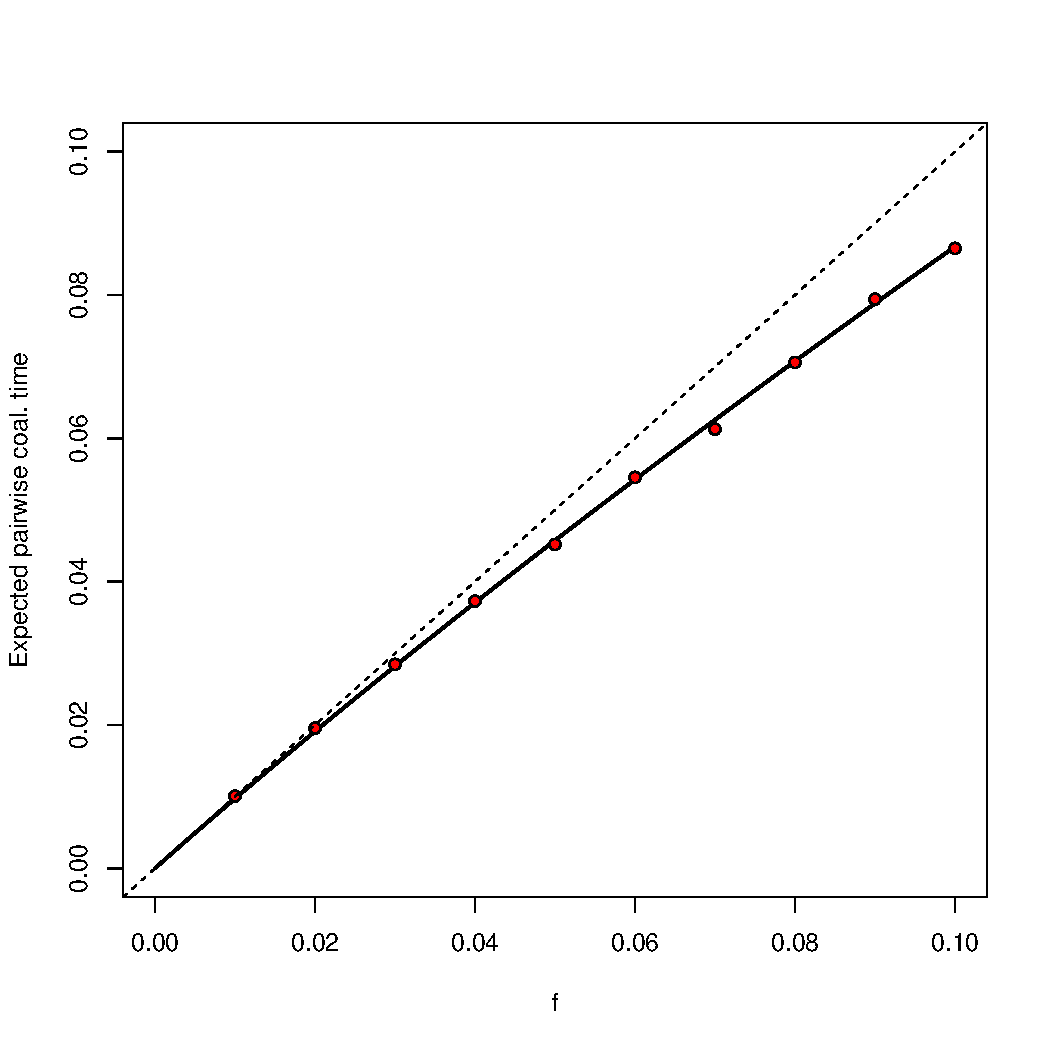
\includegraphics[width = \textwidth]{../Paper_Figures/n_two_coal_time.pdf} 
\caption{The expected pairwise coalescent time, in units of $2N$ generation, on the background of a derived neutral allele with frequency $f$ in the population.  The dashed $x=y$ line shows our approximation $\mathbb{E}  [T_2]=2Nf$. The red dots show the mean of our pairwise coalescent simulations featuring an explicit stochastic trajectories. The solid line shows the analytical expectation from XXXX  
$\mathbb{E} [T_2] \int_0^1 x/(f (x+(1-x)f))(2-f+2(1-f) \log(1-f)/f) dx $.}
\label{n_2_supp_plot}
\end{figure}   %%Made by process_f_trees.R

\begin{figure}
	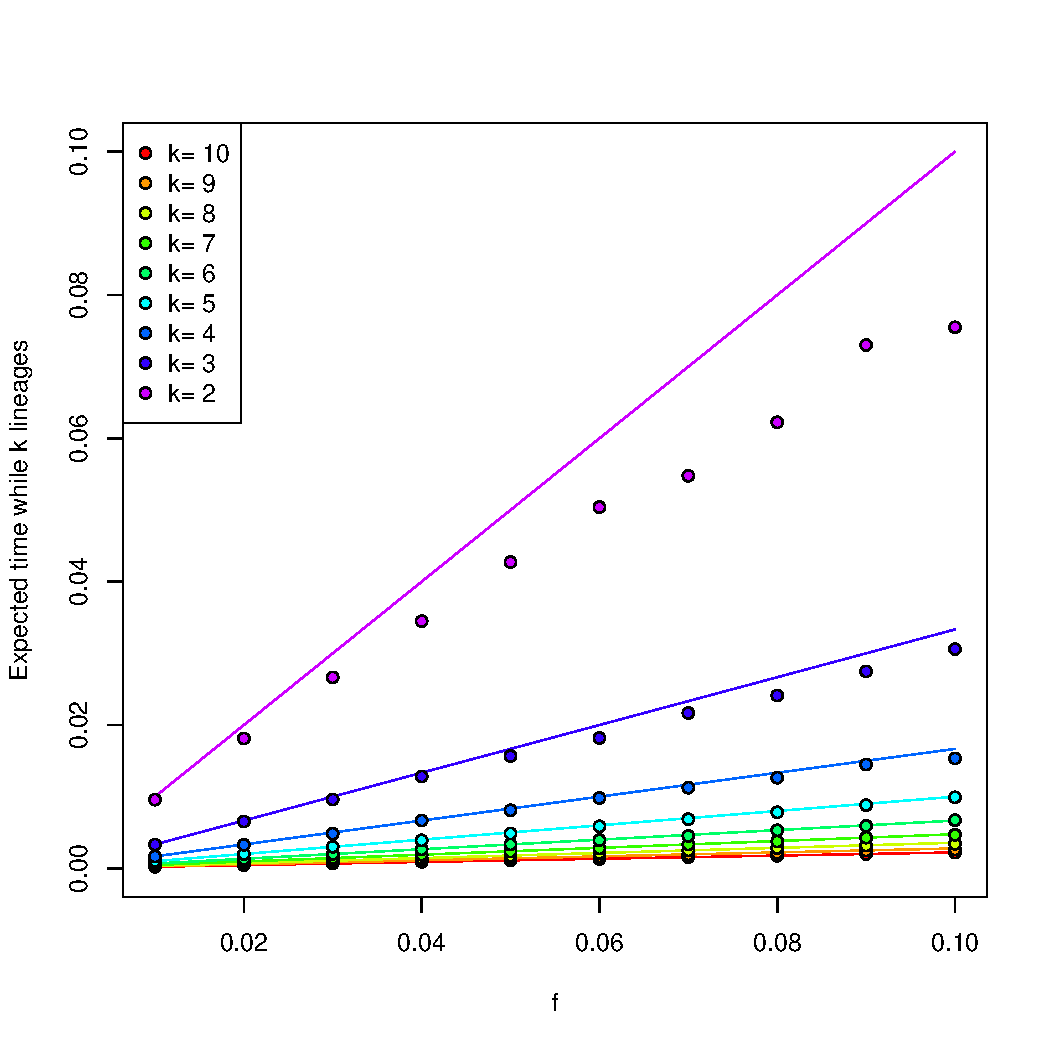
\includegraphics[width = \textwidth]{../Paper_Figures/mean_coal_times_derived.pdf} \label{mean_coal_times_supp_plot}
\caption{Expected inter-coalescent time intervals for $10$ lineages sampled in the current day on the background of a derived neutral allele with frequency $f$ in the population. 
The colored dots give means of $T_k$ from our simulations using stochastic trajectories. The solid lines show the expected coalescent times 
under our approximation $ \mathbb{E} [T_k] = 2Nf/{k \choose 2}$. Note the good agreement except for $k=2$. Presumably our approximation over estimates this time as it fails to acknowledge that the allele is derived, and hence is decreasing in frequency backward in time. }
\label{mean_coal_times_supp_plot}
\end{figure} %%Made by process_f_trees.R

\begin{figure}
	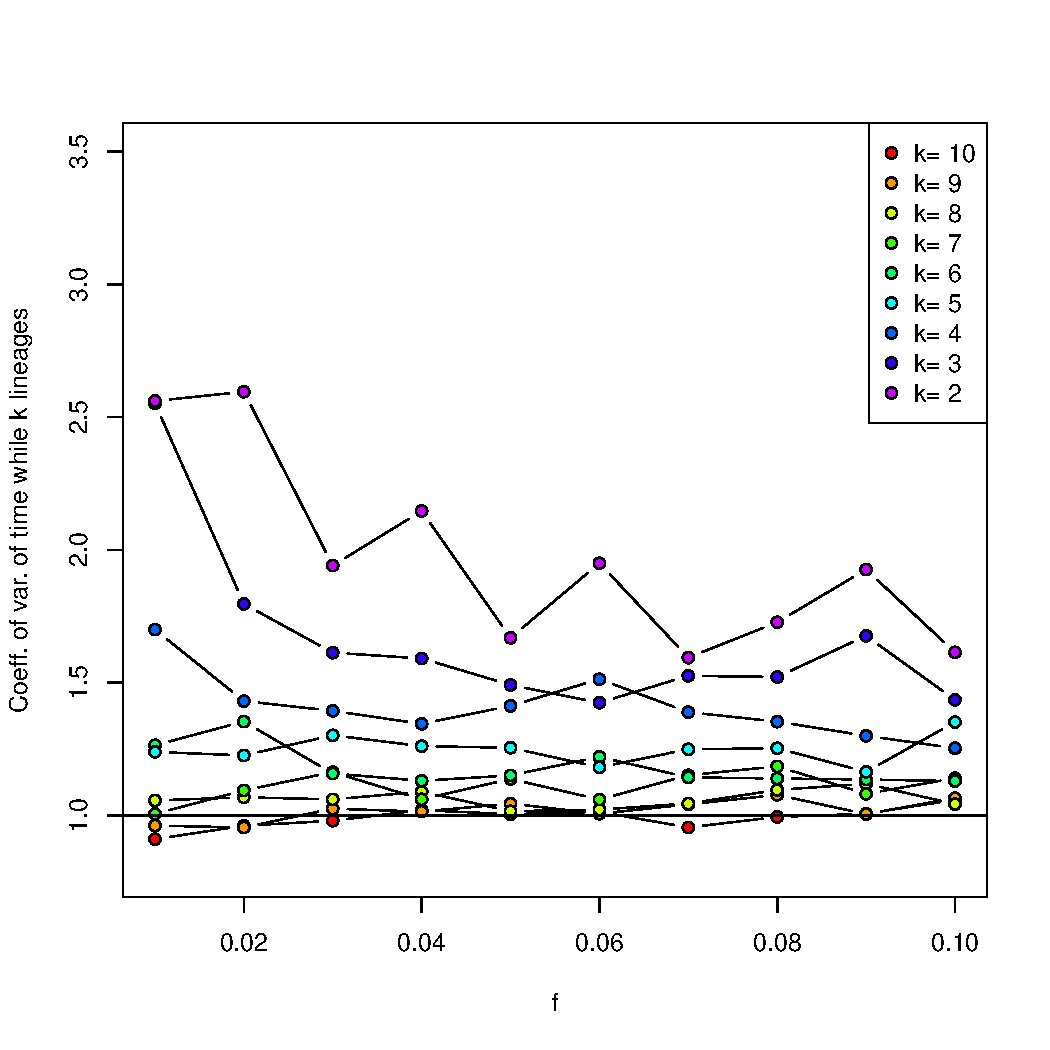
\includegraphics[width = \textwidth]{../Paper_Figures/coeff_var_coal_times.pdf} 
\caption{The coefficient of variation (CV) of the inter-coalescent time intervals for $10$ lineages sampled in the current day on the background of a derived neutral allele with frequency $f$ in the population. The colored dots give the CVs of $T_k$ from our simulations using stochastic trajectories. Under our approximation the coalescent time intervals are exponential, and so have CV=1. The deeper coalescent time-intervals (low $k$s) are more variable than our predictions presumably because neutral trajectories are highly variable so increasing the variance of the coalescent times. More recent time-intervals (high k) are in better agreement with our approximation, as the trajectory with not have strayed far from a frequency $f$ a short way back in time. }
\label{coeff_var_coal_times_supp_plot}
\end{figure} %%Made by process_f_trees.R

\end{document}
